\chapter{MODFLOW - Additional model results}
\label{chapter:MODFLOW_additional}

\section{ASR system base model performance}
\label{section:base_performance}

Figure \ref{fig:Example_Sc3_base_head_wet} illustrates the precise impact of flood based ASR-system infiltration on soil scenario 3 groundwater heads in several representative (model) layers. Worth mentioning, groundwater level increase is already limited at relative short radial distance (steep groundwater cone).   

\begin{figure}[h!]
	\centering
	\begin{subfigure}[b]{0.5\linewidth}
		\centering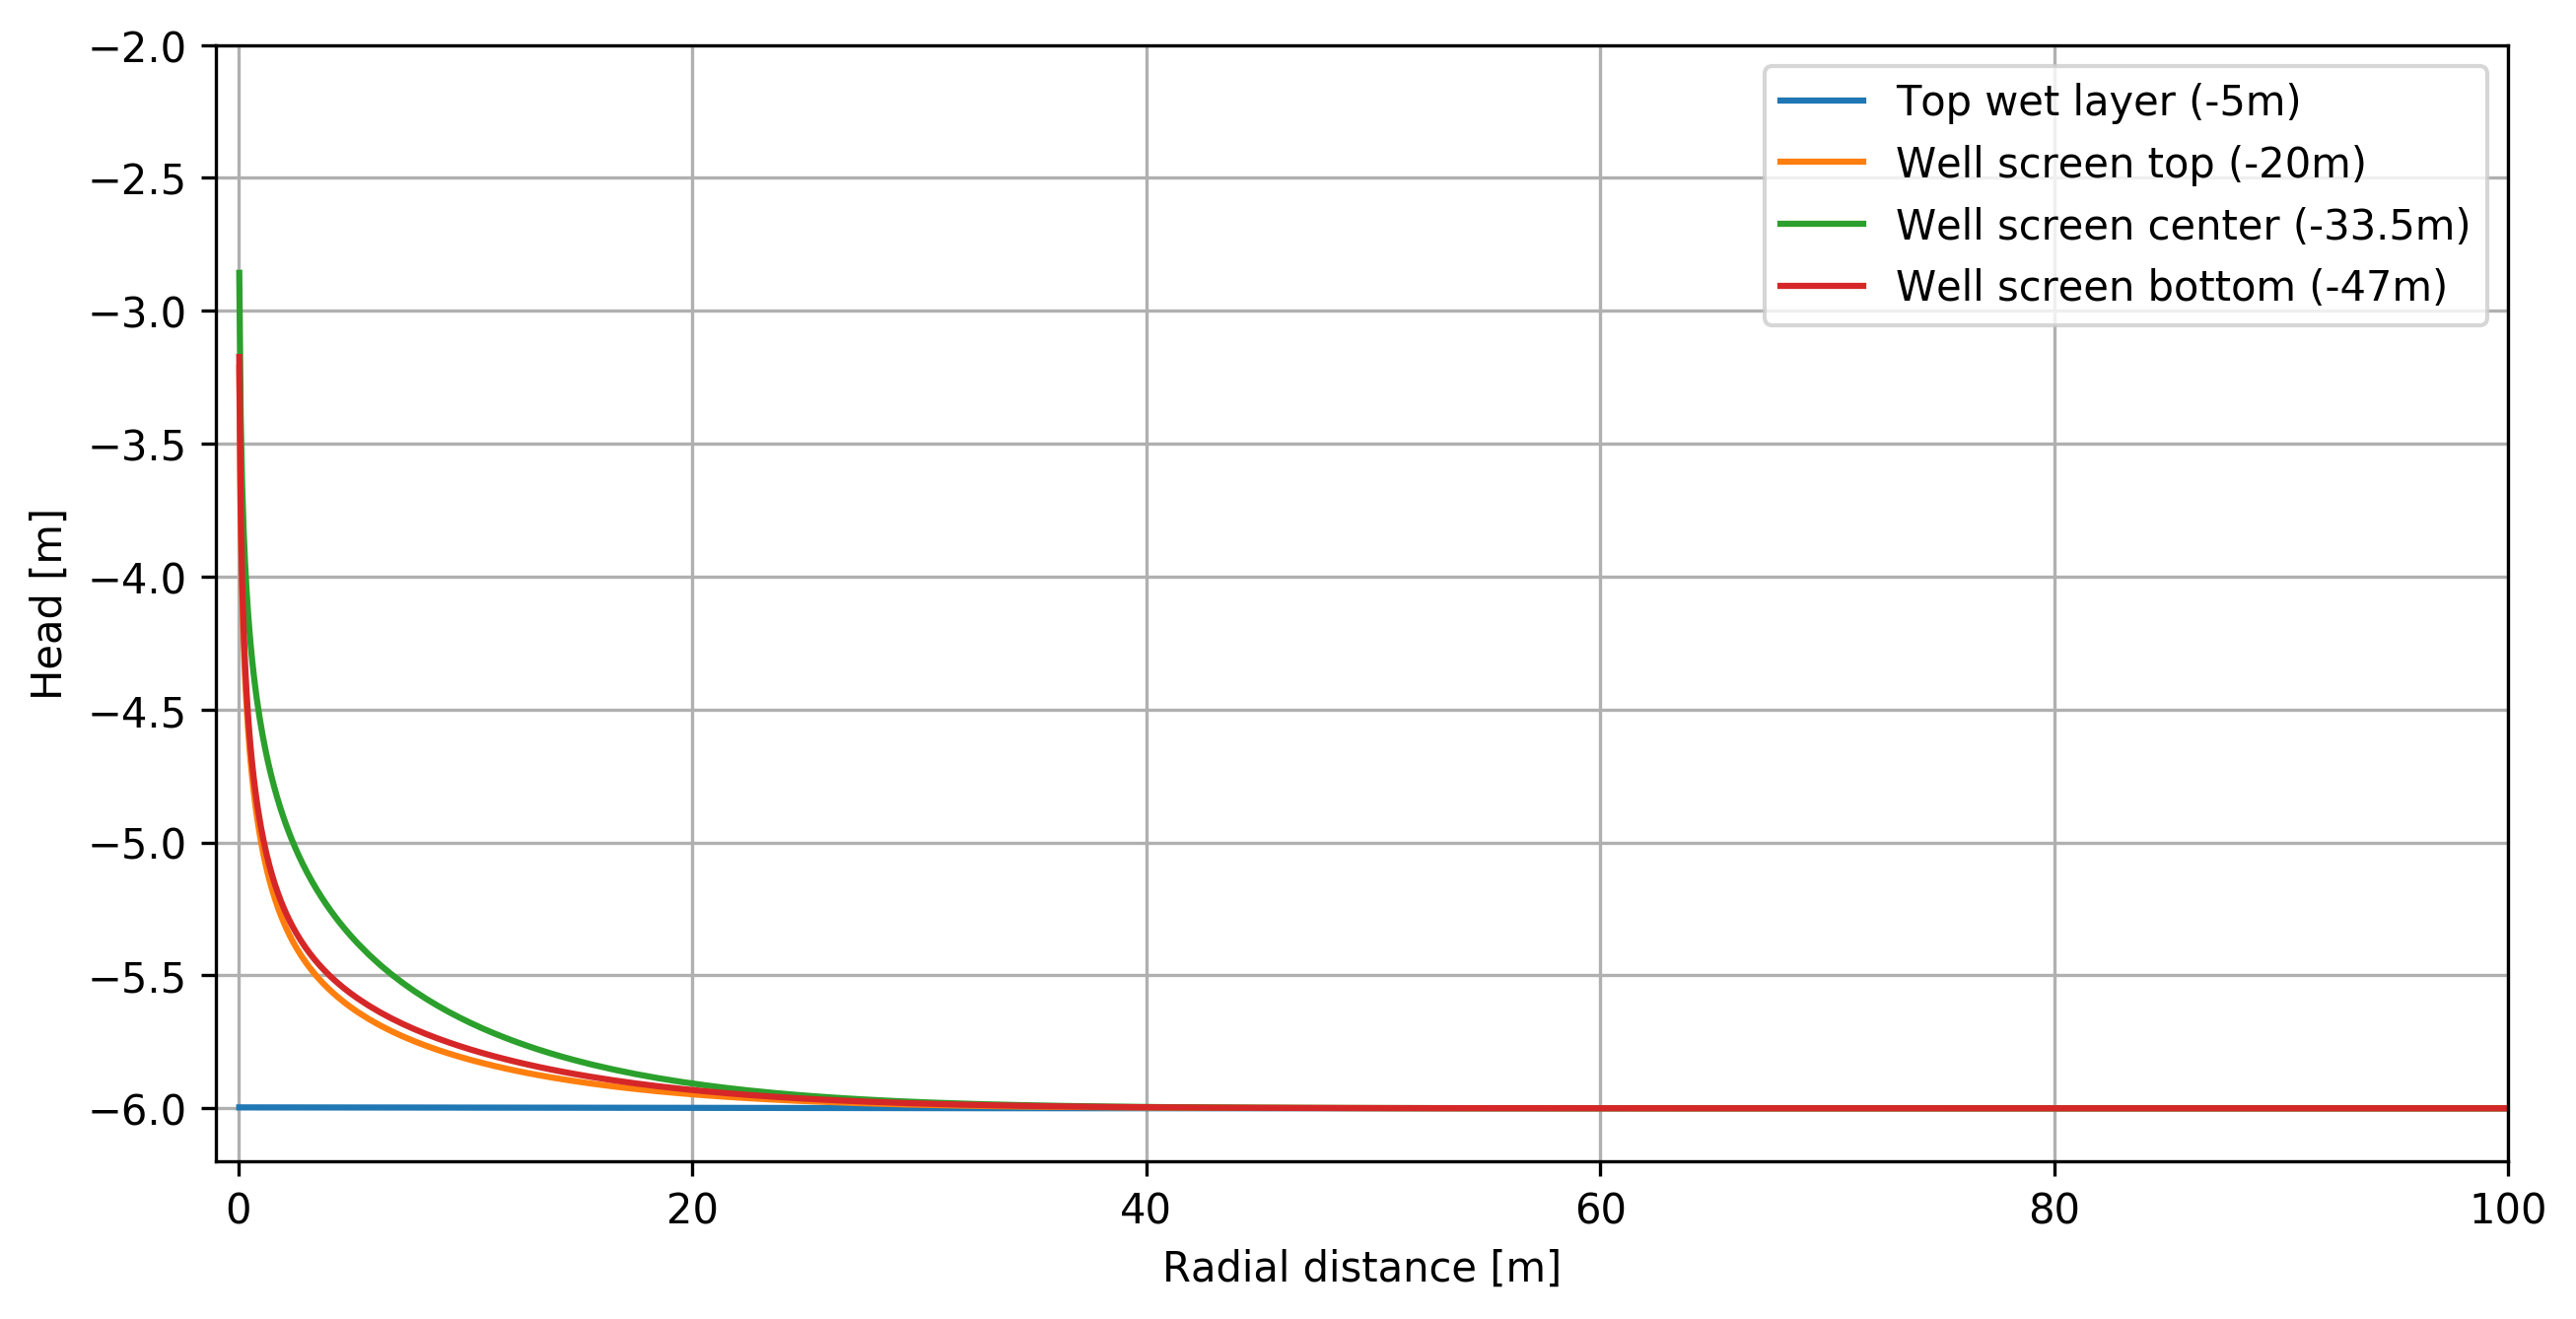
\includegraphics[width=\linewidth]{Sc3a1_head_d5}
		\captionsetup{justification=centering}		
		\caption{\label{fig:Sc3a1_head_d5}}
		\end{subfigure}\hfill
	\begin{subfigure}[b]{0.5\linewidth}
        \centering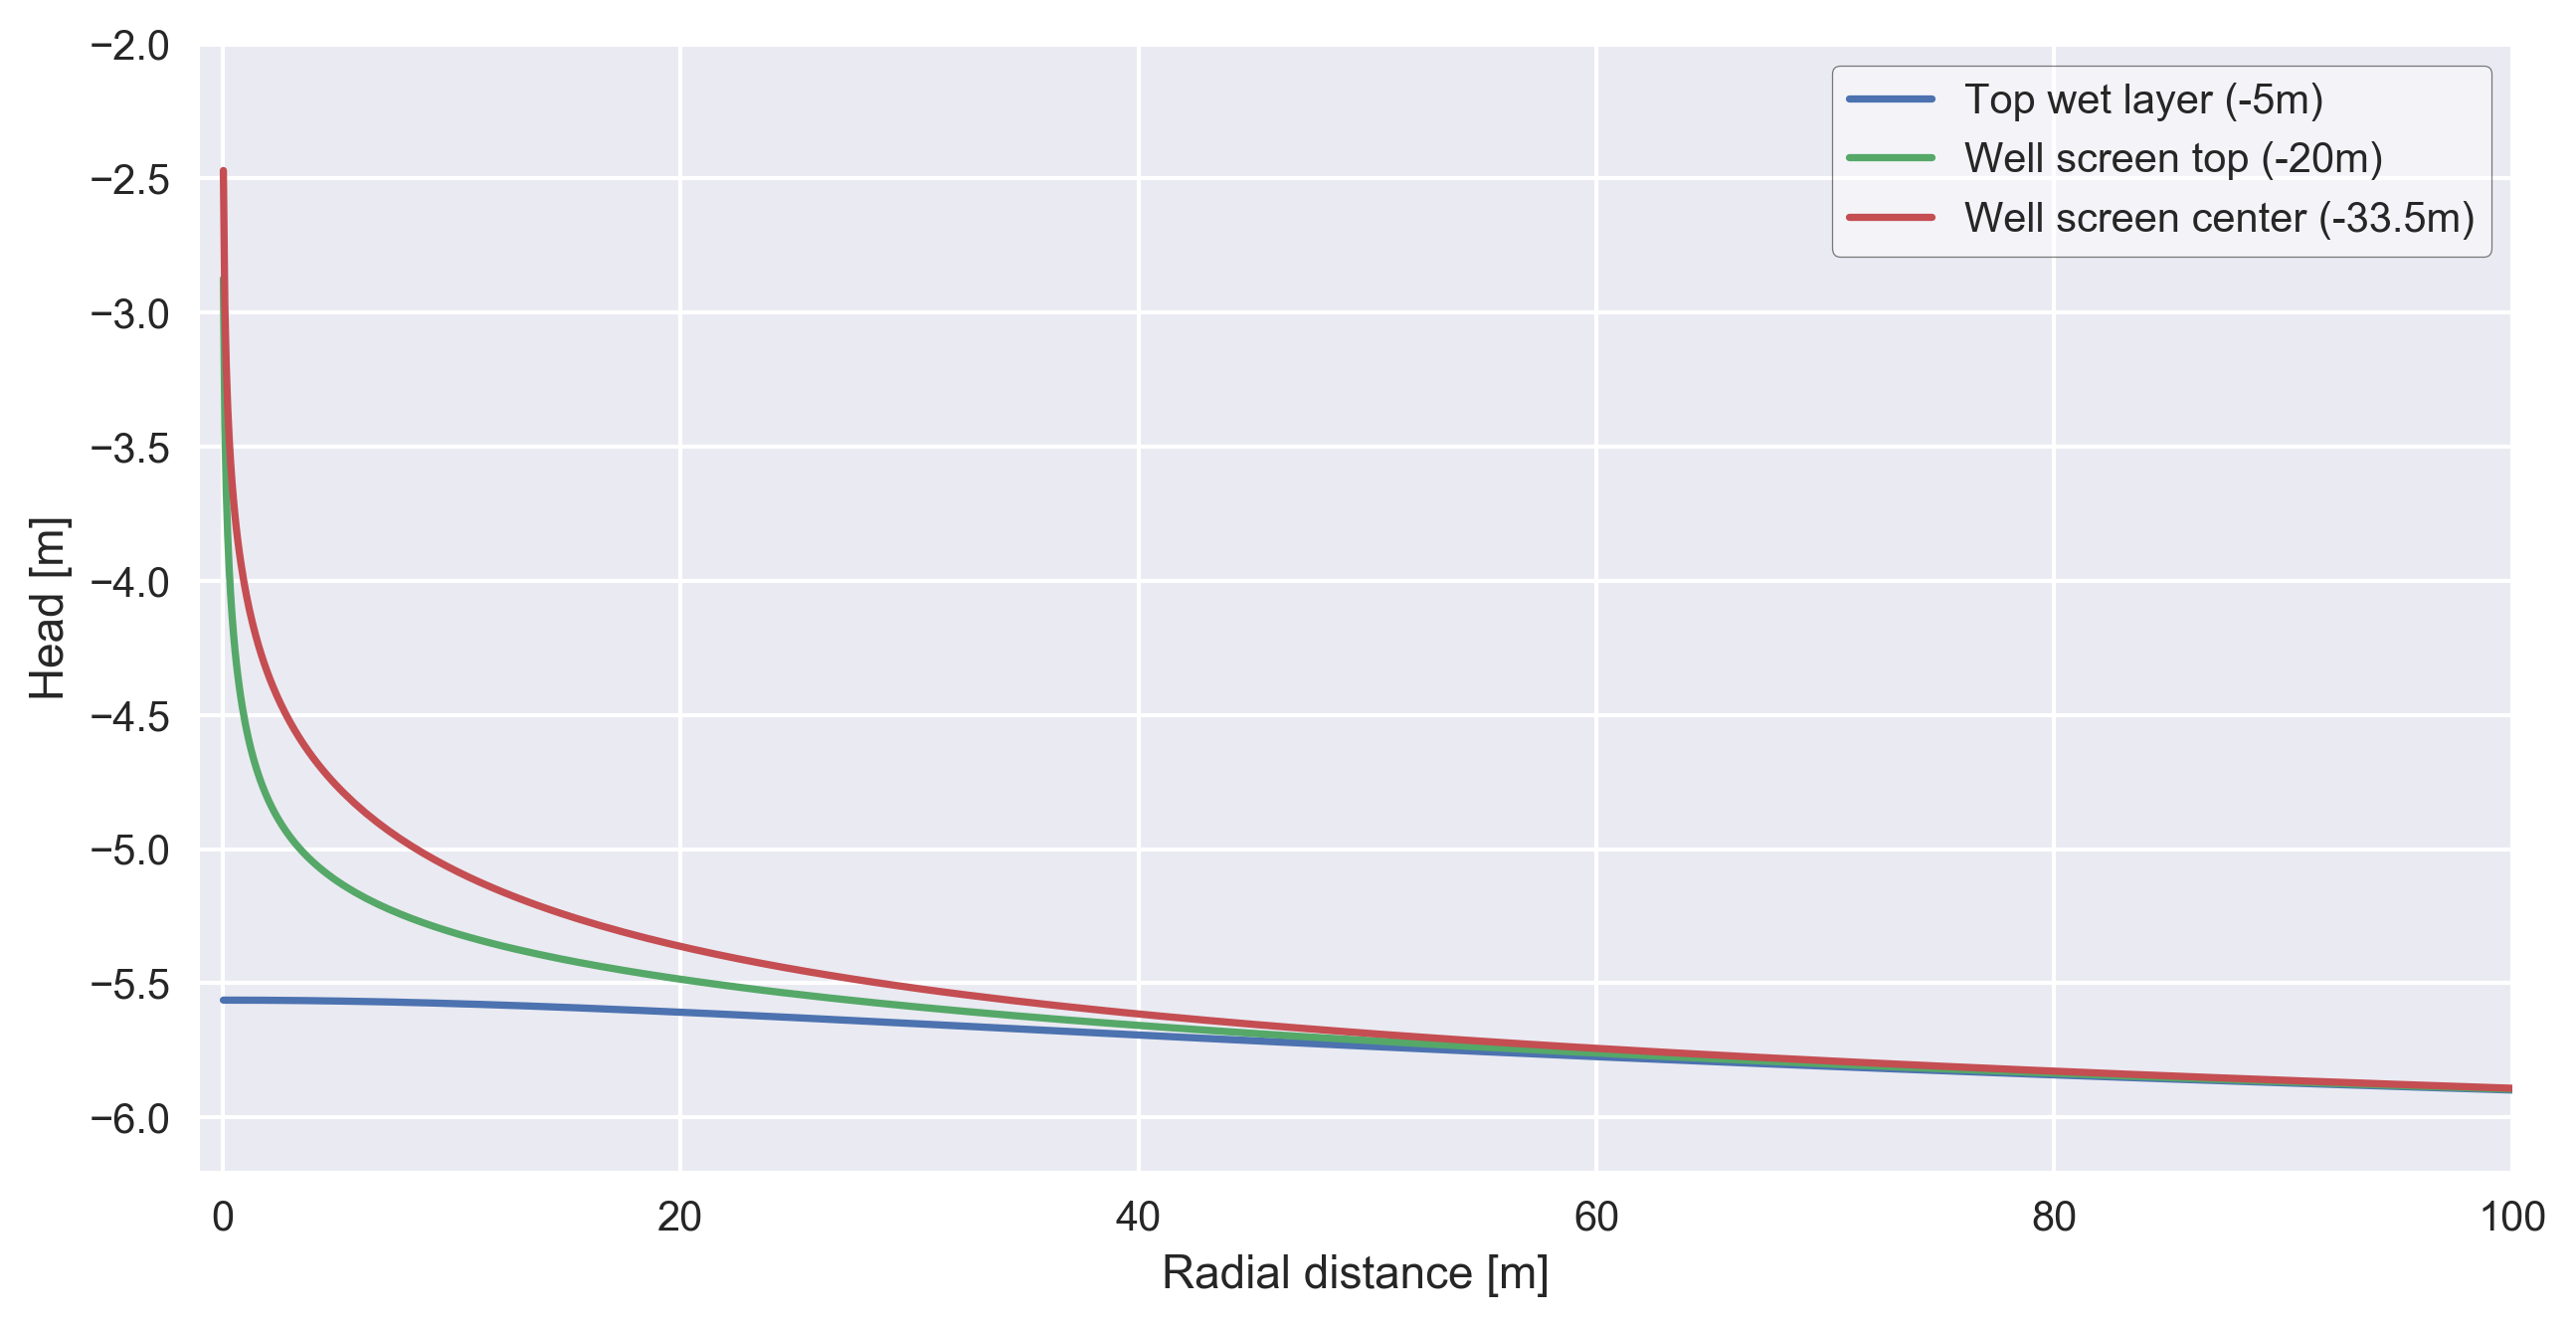
\includegraphics[width=\linewidth]{Sc3a1_head_d122}
		\captionsetup{justification=centering}		
		\caption{\label{fig:Sc3a1_head_d122}}
		\end{subfigure}
		\captionsetup{justification=centering}	
	\caption{Base model soil scenario 3 - Head in representative layers after (\subref{fig:Sc3a1_head_d5}) five days and (\subref{fig:Sc3a1_head_d122}) 122 days of infiltration} 
	\label{fig:Example_Sc3_base_head_wet}
\end{figure} 

Figure \ref{fig:Example_Sc3_base_head_dry} presents the precise impact of discharge on soil scenario 3 groundwater heads in several representative (model) layers. After the first day of pumping the transition from wet (recharge) to dry season (discharge) is still of influence. Most definitely in the higher model layers (close to surface) the increased heads (due to wet season recharge) remain active for some time. Towards the end of dry season this impact is no longer present.

\begin{figure}[h!]
	\centering
	\begin{subfigure}[b]{0.5\linewidth}
		\centering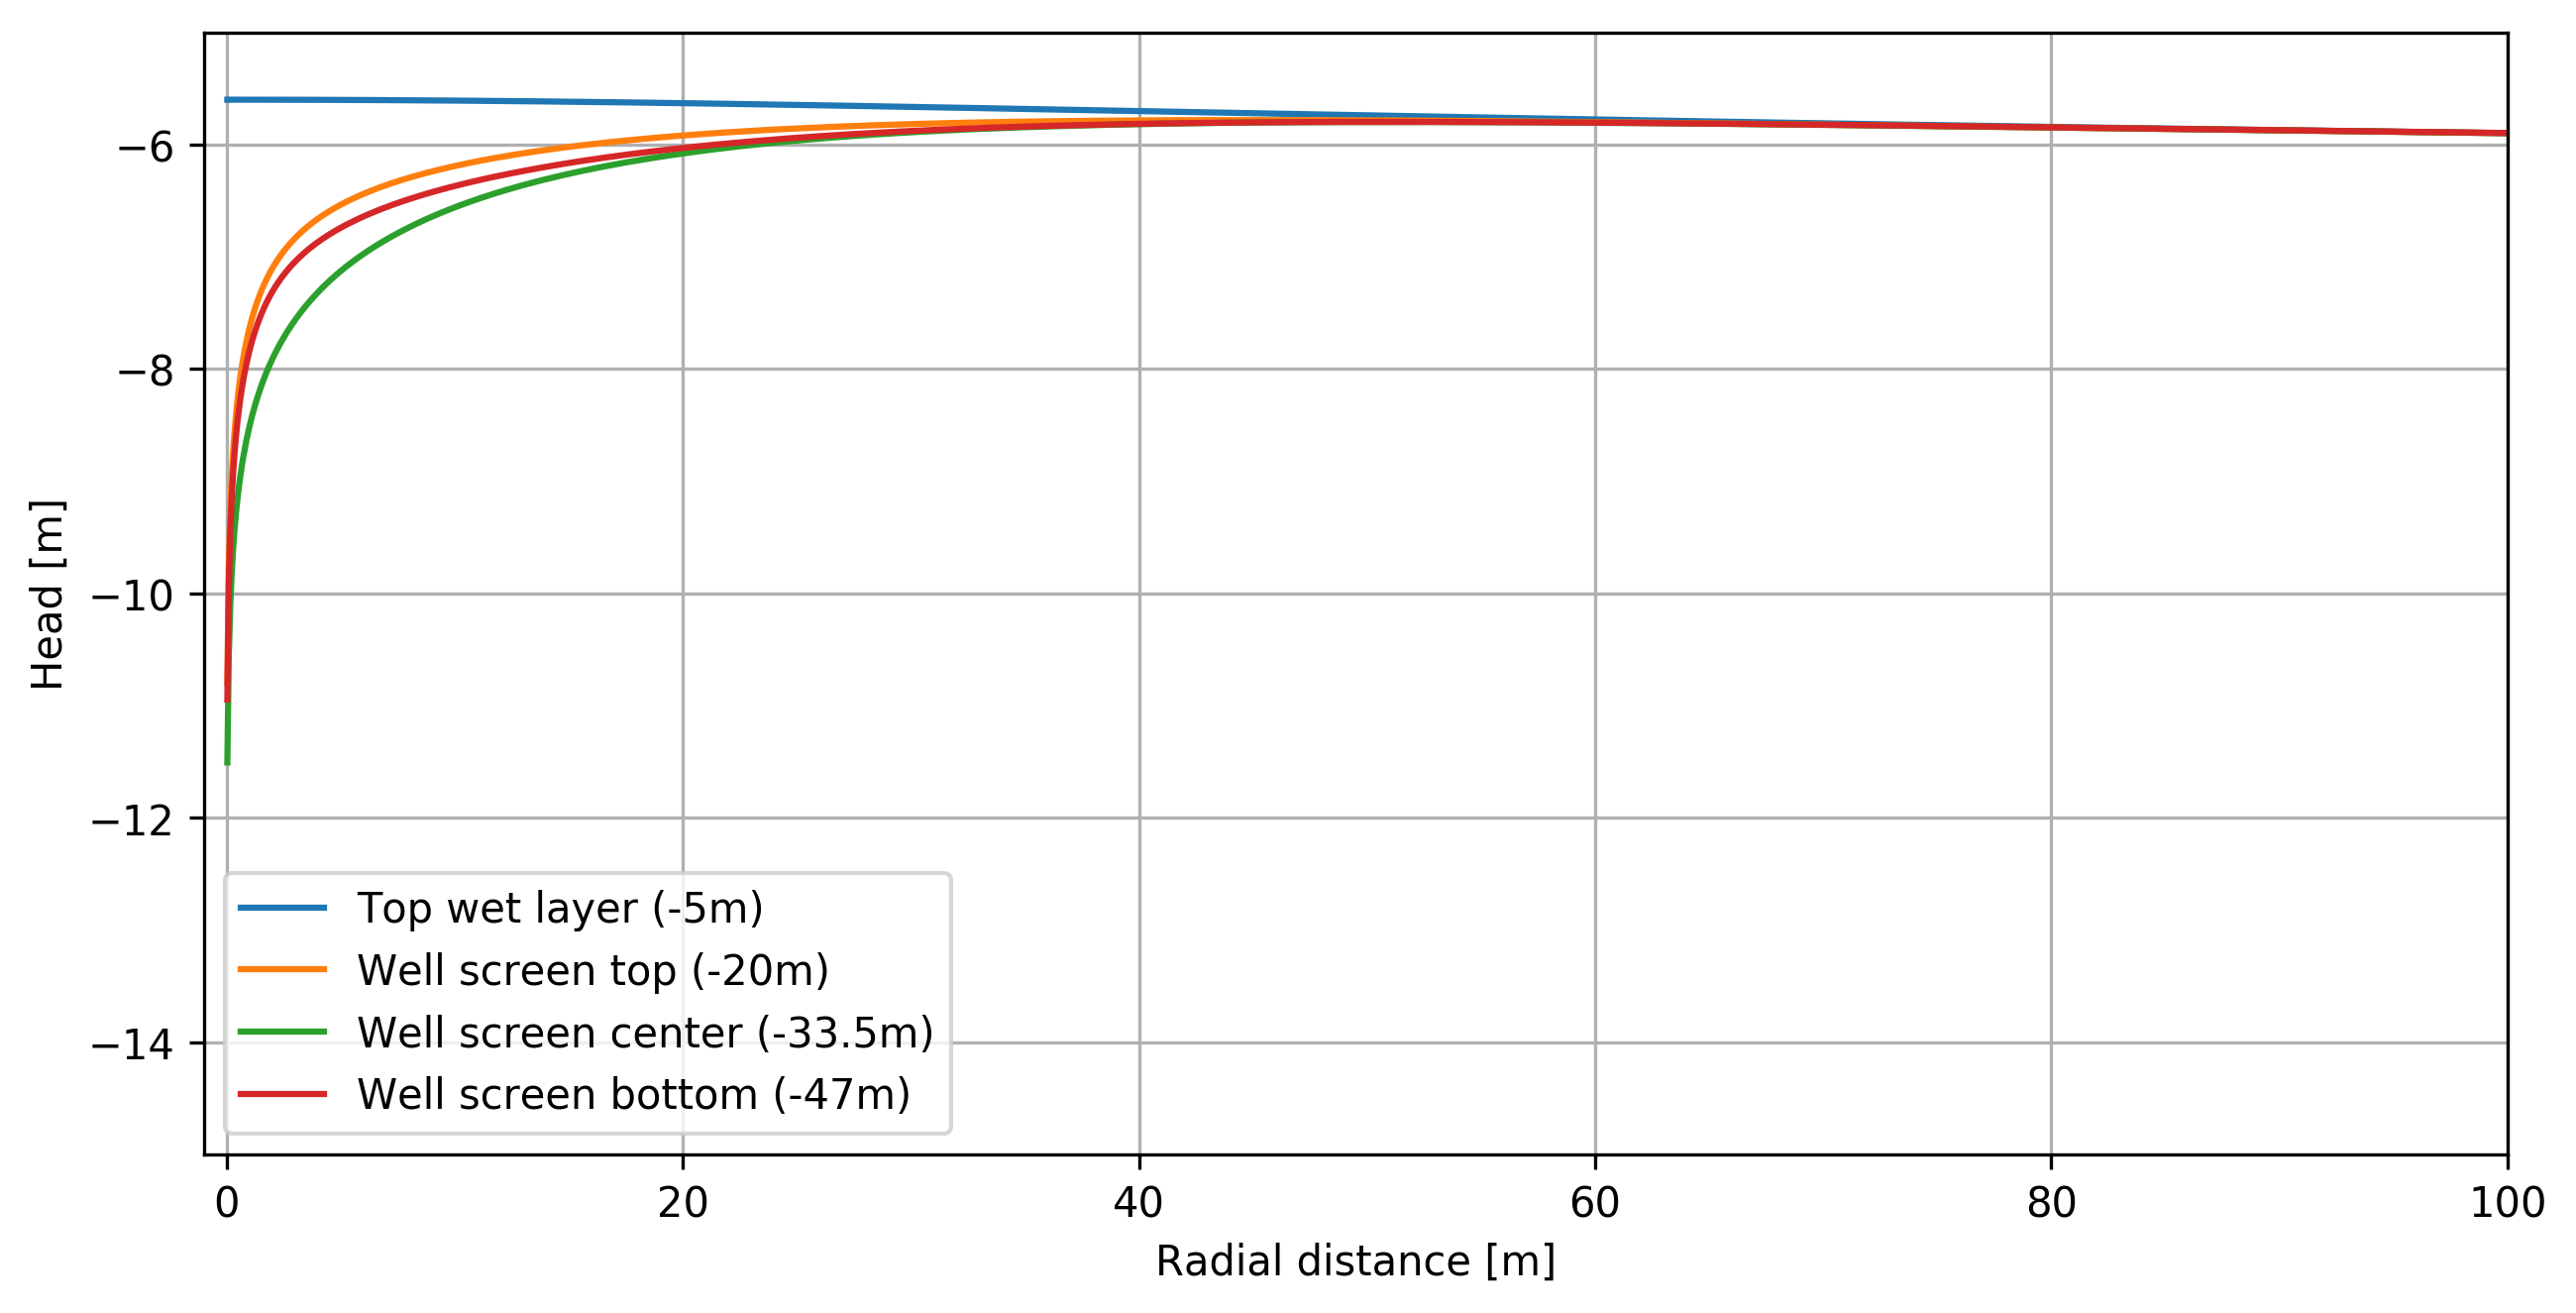
\includegraphics[width=\linewidth]{Sc3a1_head_d123pump}
		\captionsetup{justification=centering}		
		\caption{\label{fig:Sc3a1_head_d123pump}}
		\end{subfigure}\hfill
	\begin{subfigure}[b]{0.5\linewidth}
        \centering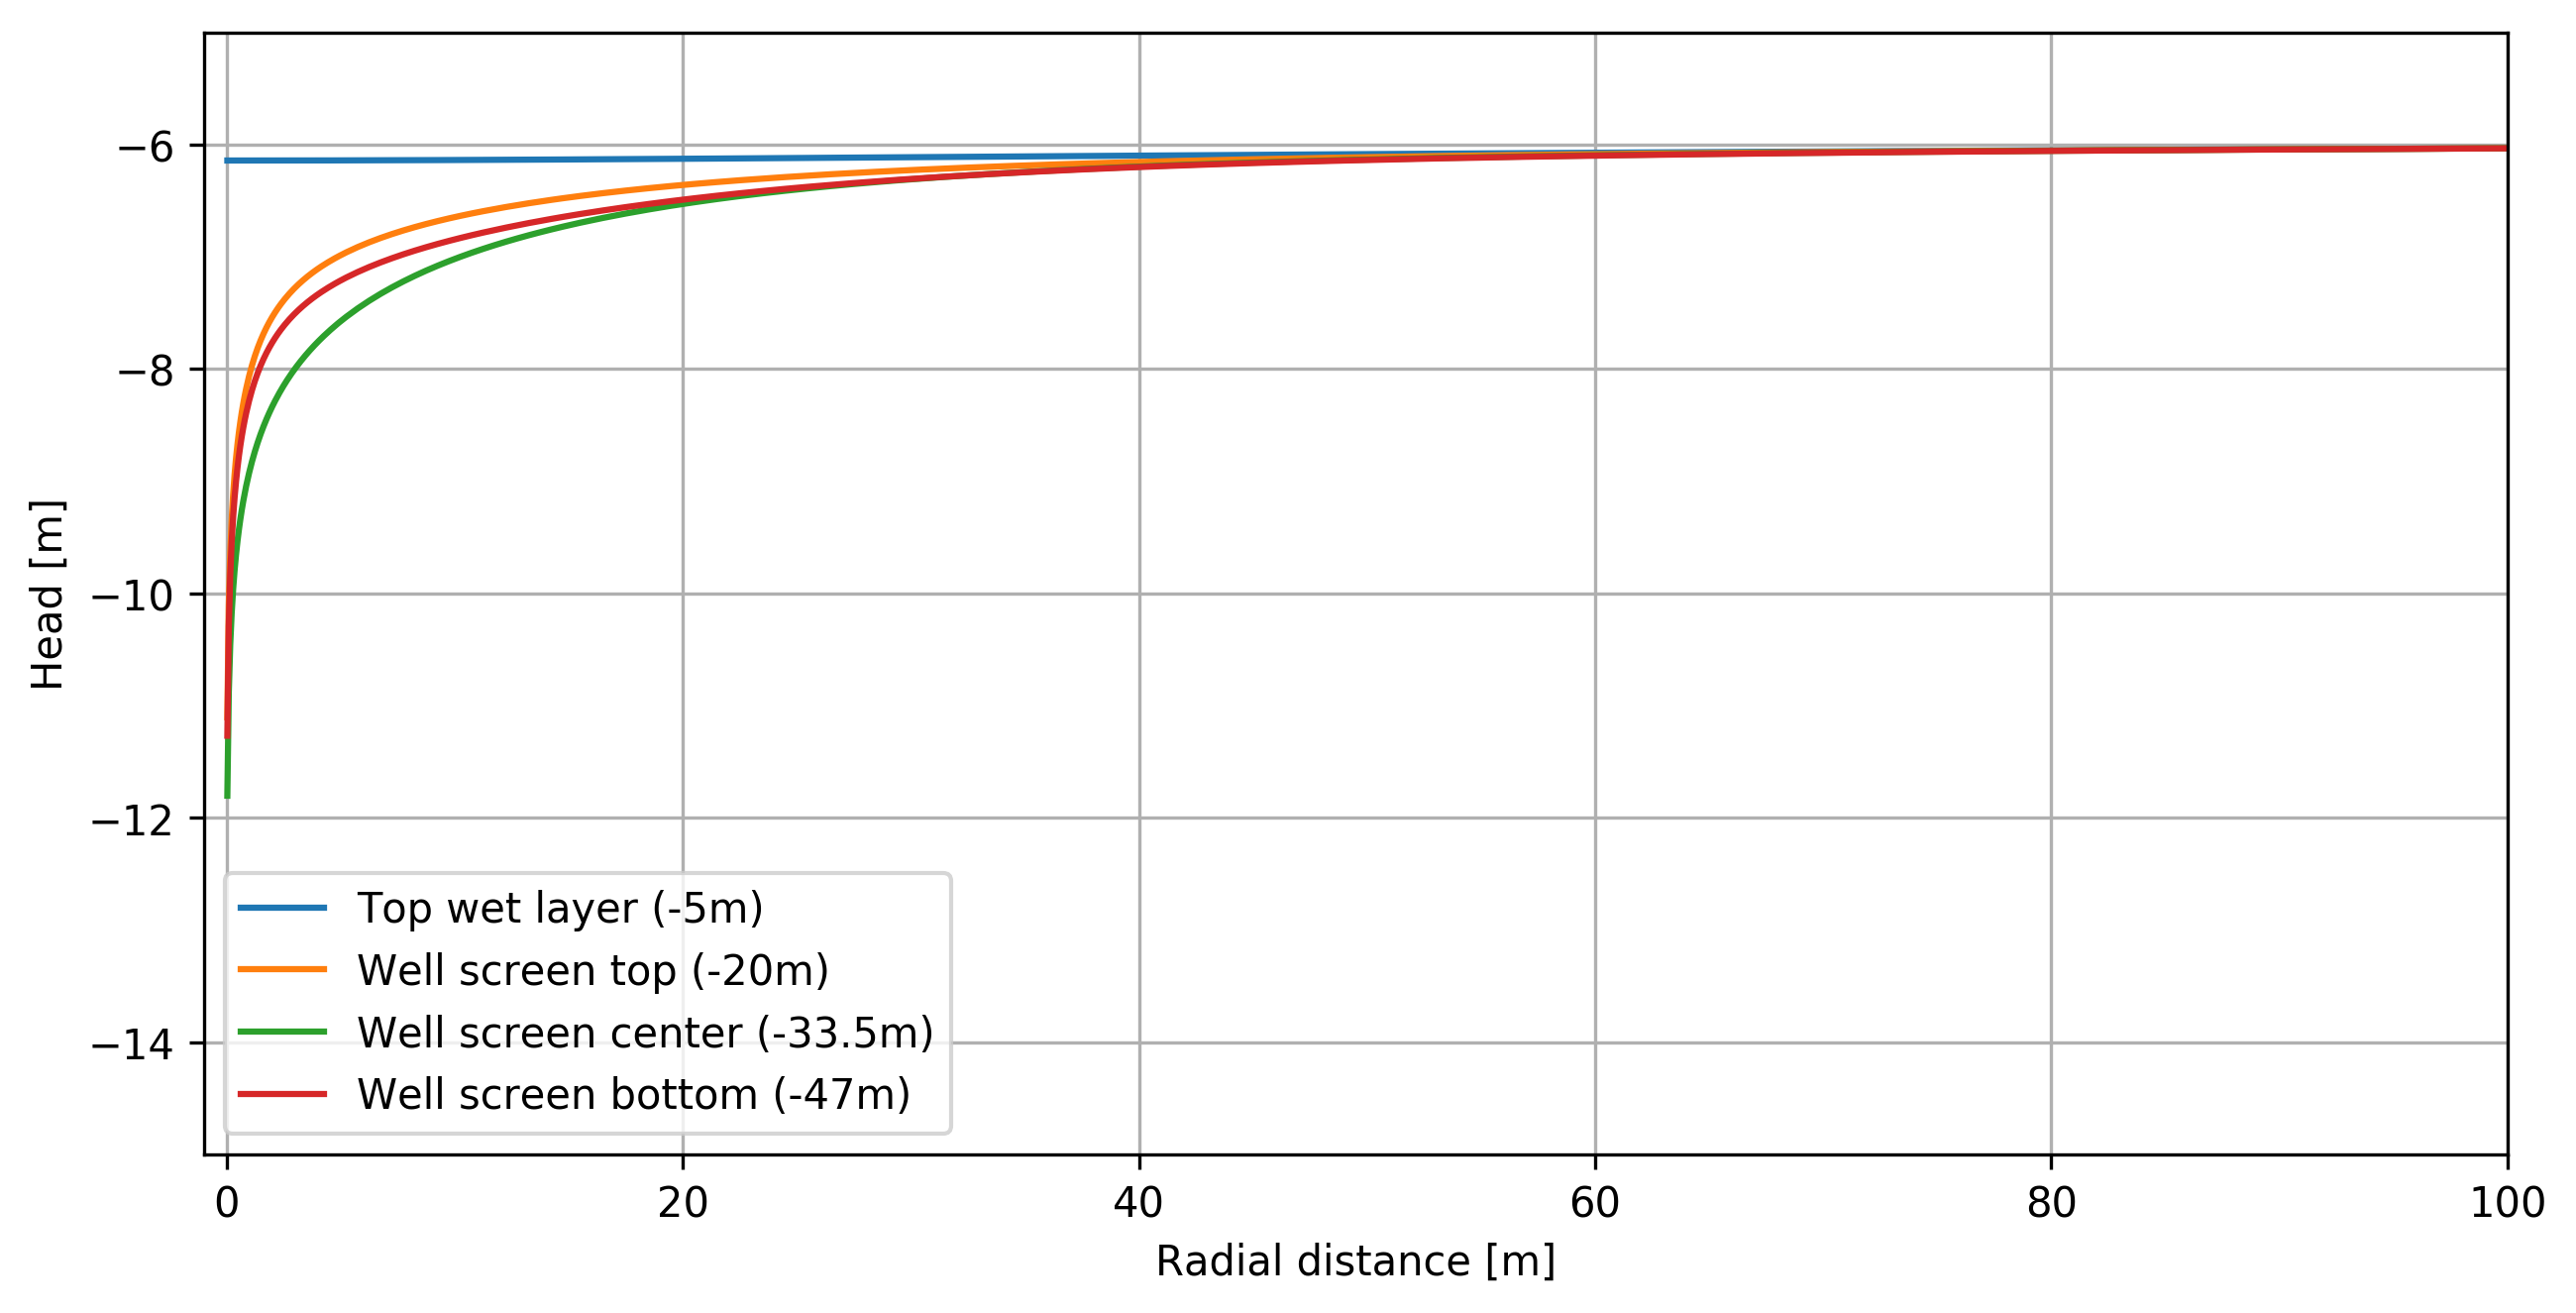
\includegraphics[width=\linewidth]{Sc3a1_head_d364pump}
		\captionsetup{justification=centering}		
		\caption{\label{fig:Sc3a1_head_d364pump}}
		\end{subfigure}
		\captionsetup{justification=centering}	
	\caption{Base model soil scenario 3 - Head in representative layers after four hours of pumping on (\subref{fig:Sc3a1_head_d123pump}) the first day (day 123) and (\subref{fig:Sc3a1_head_d364pump}) the last day (day 365) of dry season} 
	\label{fig:Example_Sc3_base_head_dry}
\end{figure} 

\section{ASR system sensitivity}
\label{section:addition_sens}


\begin{table}[h!]
\small
\centering
\caption{Degradation of well depth - soil scenario 3 - Screen average specific recharge and discharge volumes (m$^3$/m)}
\label{tab:sc3_up_clean_rev_specific_volume}
\begin{tabular}{l|r|r|r|r|r}
\hline 
\textbf{Screen length (m)}                   & \textbf{30}      & \textbf{25}      & \textbf{20}      & \textbf{15}      & \textbf{10}       \\ \hline \hline
Average specific recharge volume (m$^3$/m)   & 195.23  & 199.98  & 203.57  & 207.58  & 212.96   \\ \hline 
Average specific discharge volume (m$^3$/m)  & 121.03  & 122.67  & 123.65  & 124.89  & 126.85   \\ \hline     
\end{tabular}
\end{table}

\begin{table}[h!]
\small
\centering
\caption{Degradation of well depth - soil scenario 3 - Total recharge and discharge volumes specific reduction (m$^3$/m)}
\label{tab:sc3_up_clean_rev_specific_volume_reduction}
\begin{tabular}{l|r|r|r|r}
\hline 
\textbf{Reduction screen length (m)}                 & \textbf{5}      & \textbf{10}      & \textbf{15}      & \textbf{20}       \\ \hline \hline
Total recharge volume specific reduction (m$^3$/m)   & 171.47  & 178.54  & 182.87  & 186.36    \\ \hline 
Total discharge volume specific reduction (m$^3$/m)  & 112.84  & 115.78  & 117.17  & 118.12    \\ \hline     
\end{tabular}
\end{table}


\begin{figure}[h!]
 \centering
 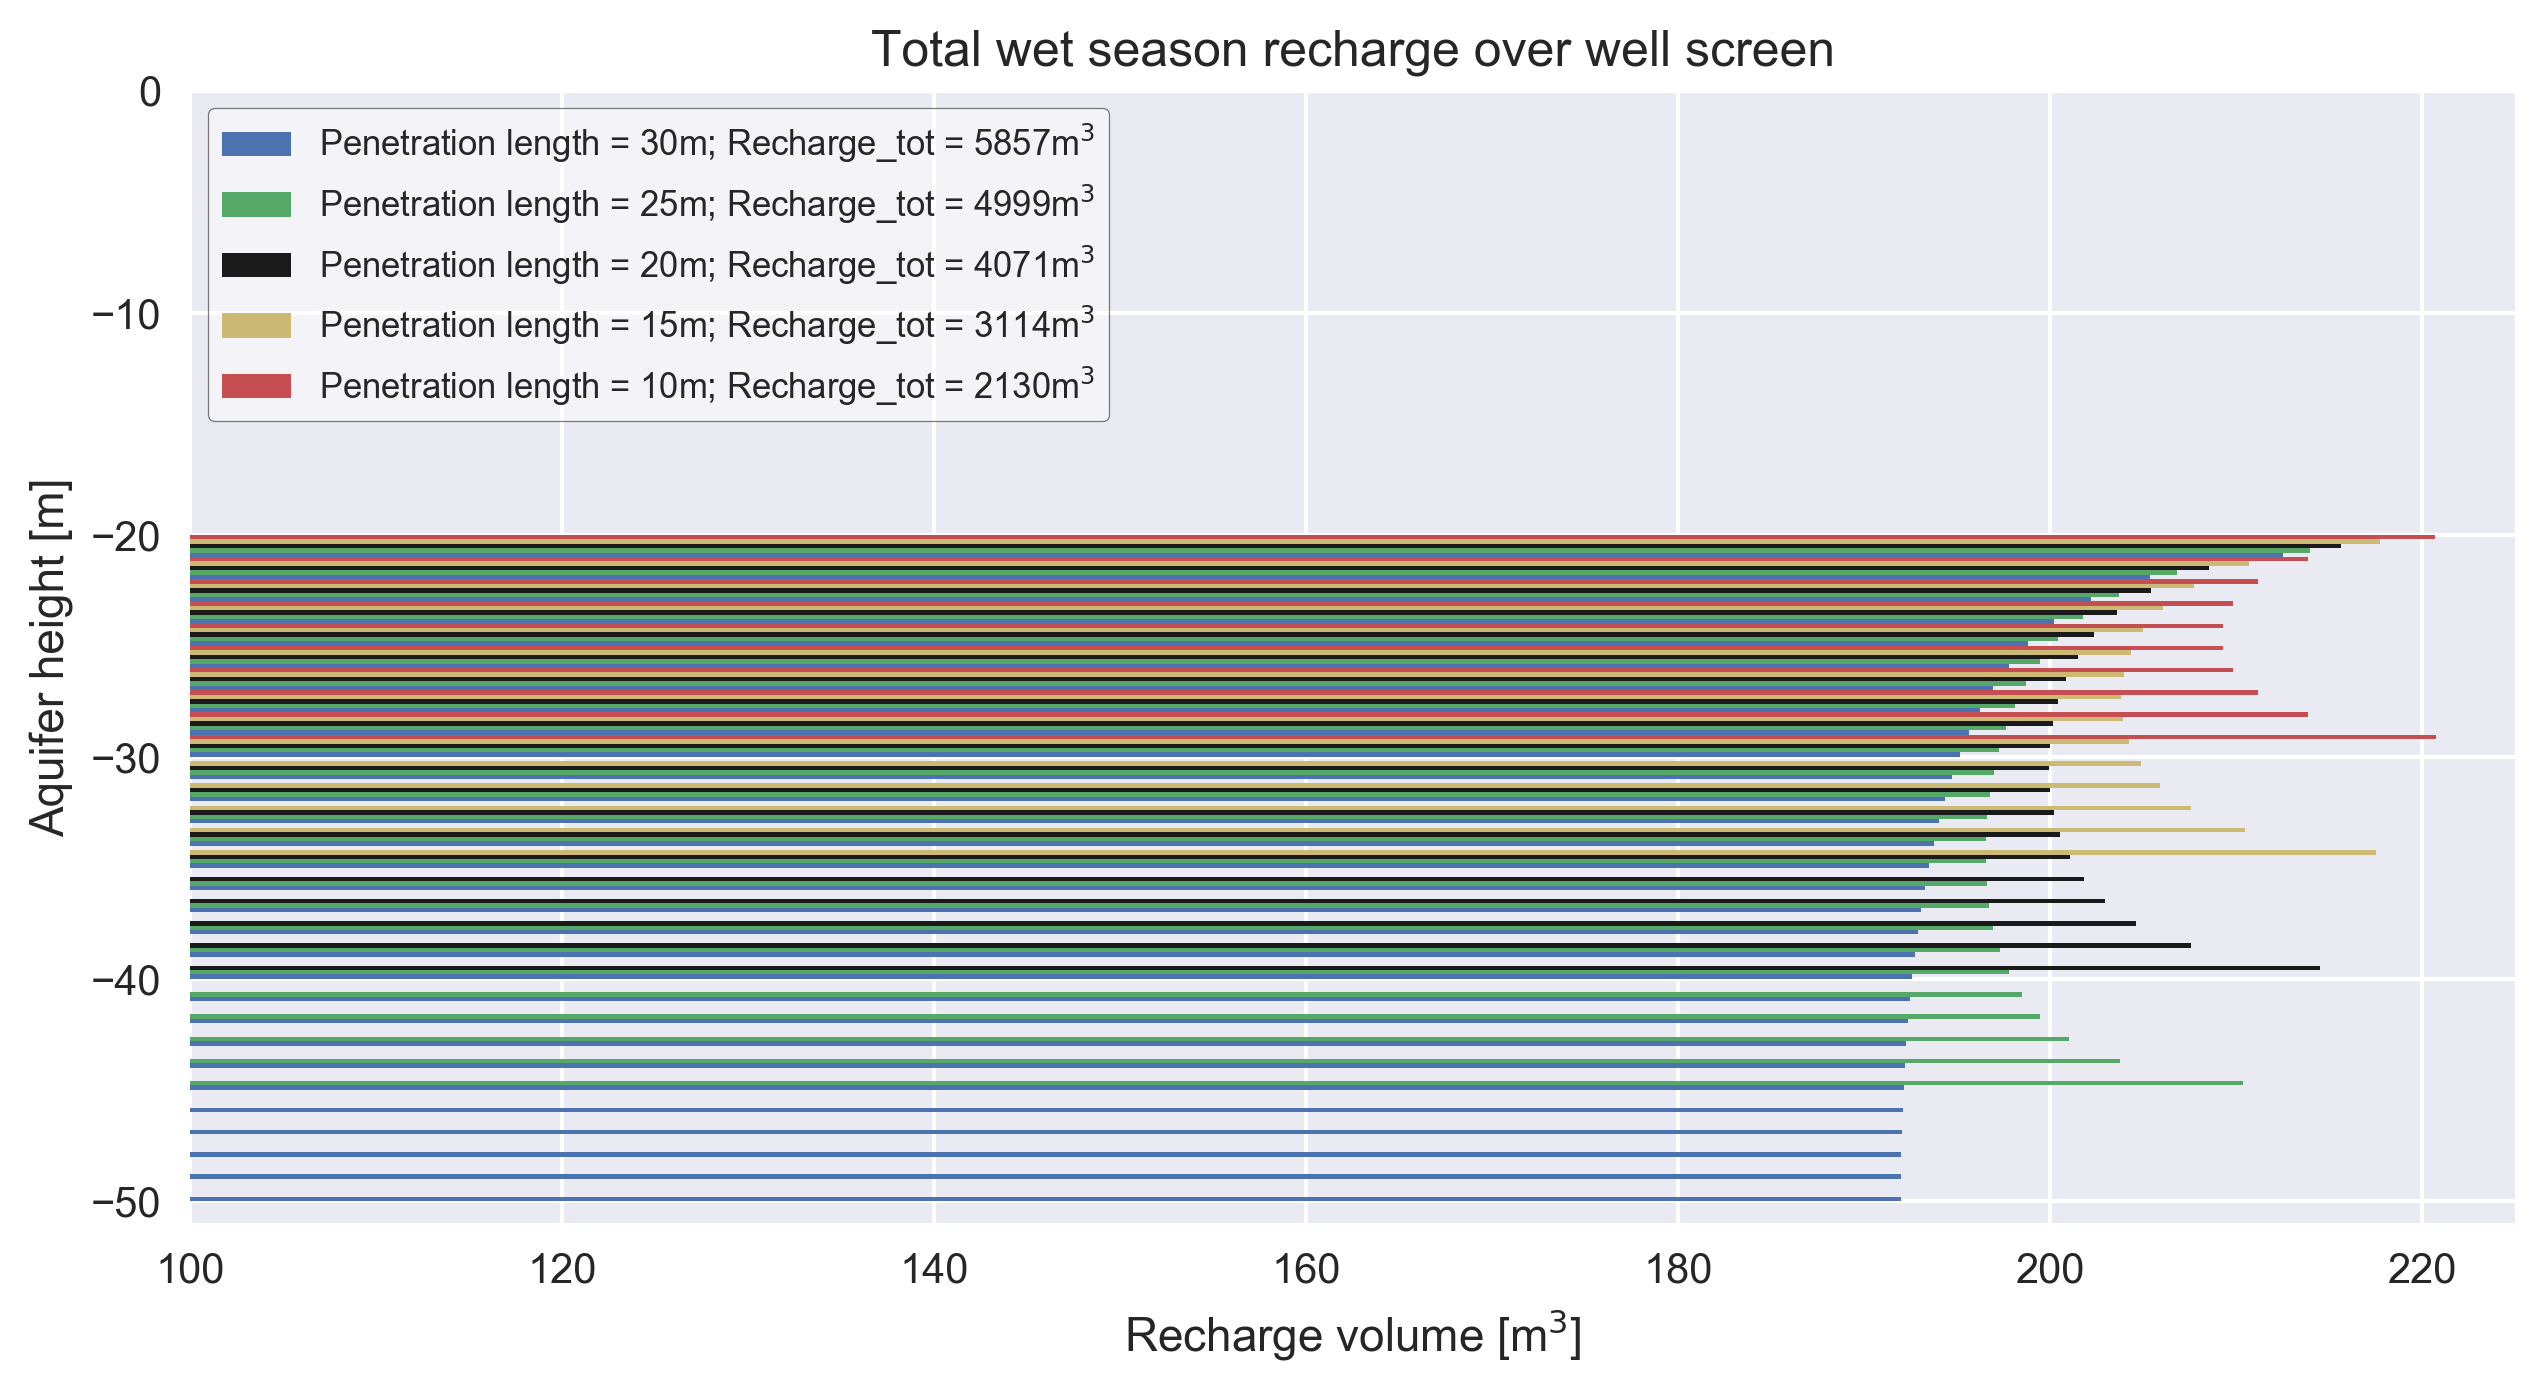
\includegraphics[width=0.7\linewidth]{Sc3c_recharge_layers}
 \captionsetup{justification=centering} 
 \caption{Degradation of well depth - Total recharge volume by layer - soil scenario 3}
 \label{fig:Sc3c_recharge_layers}
\end{figure}


\begin{figure}[h!]
 \centering
 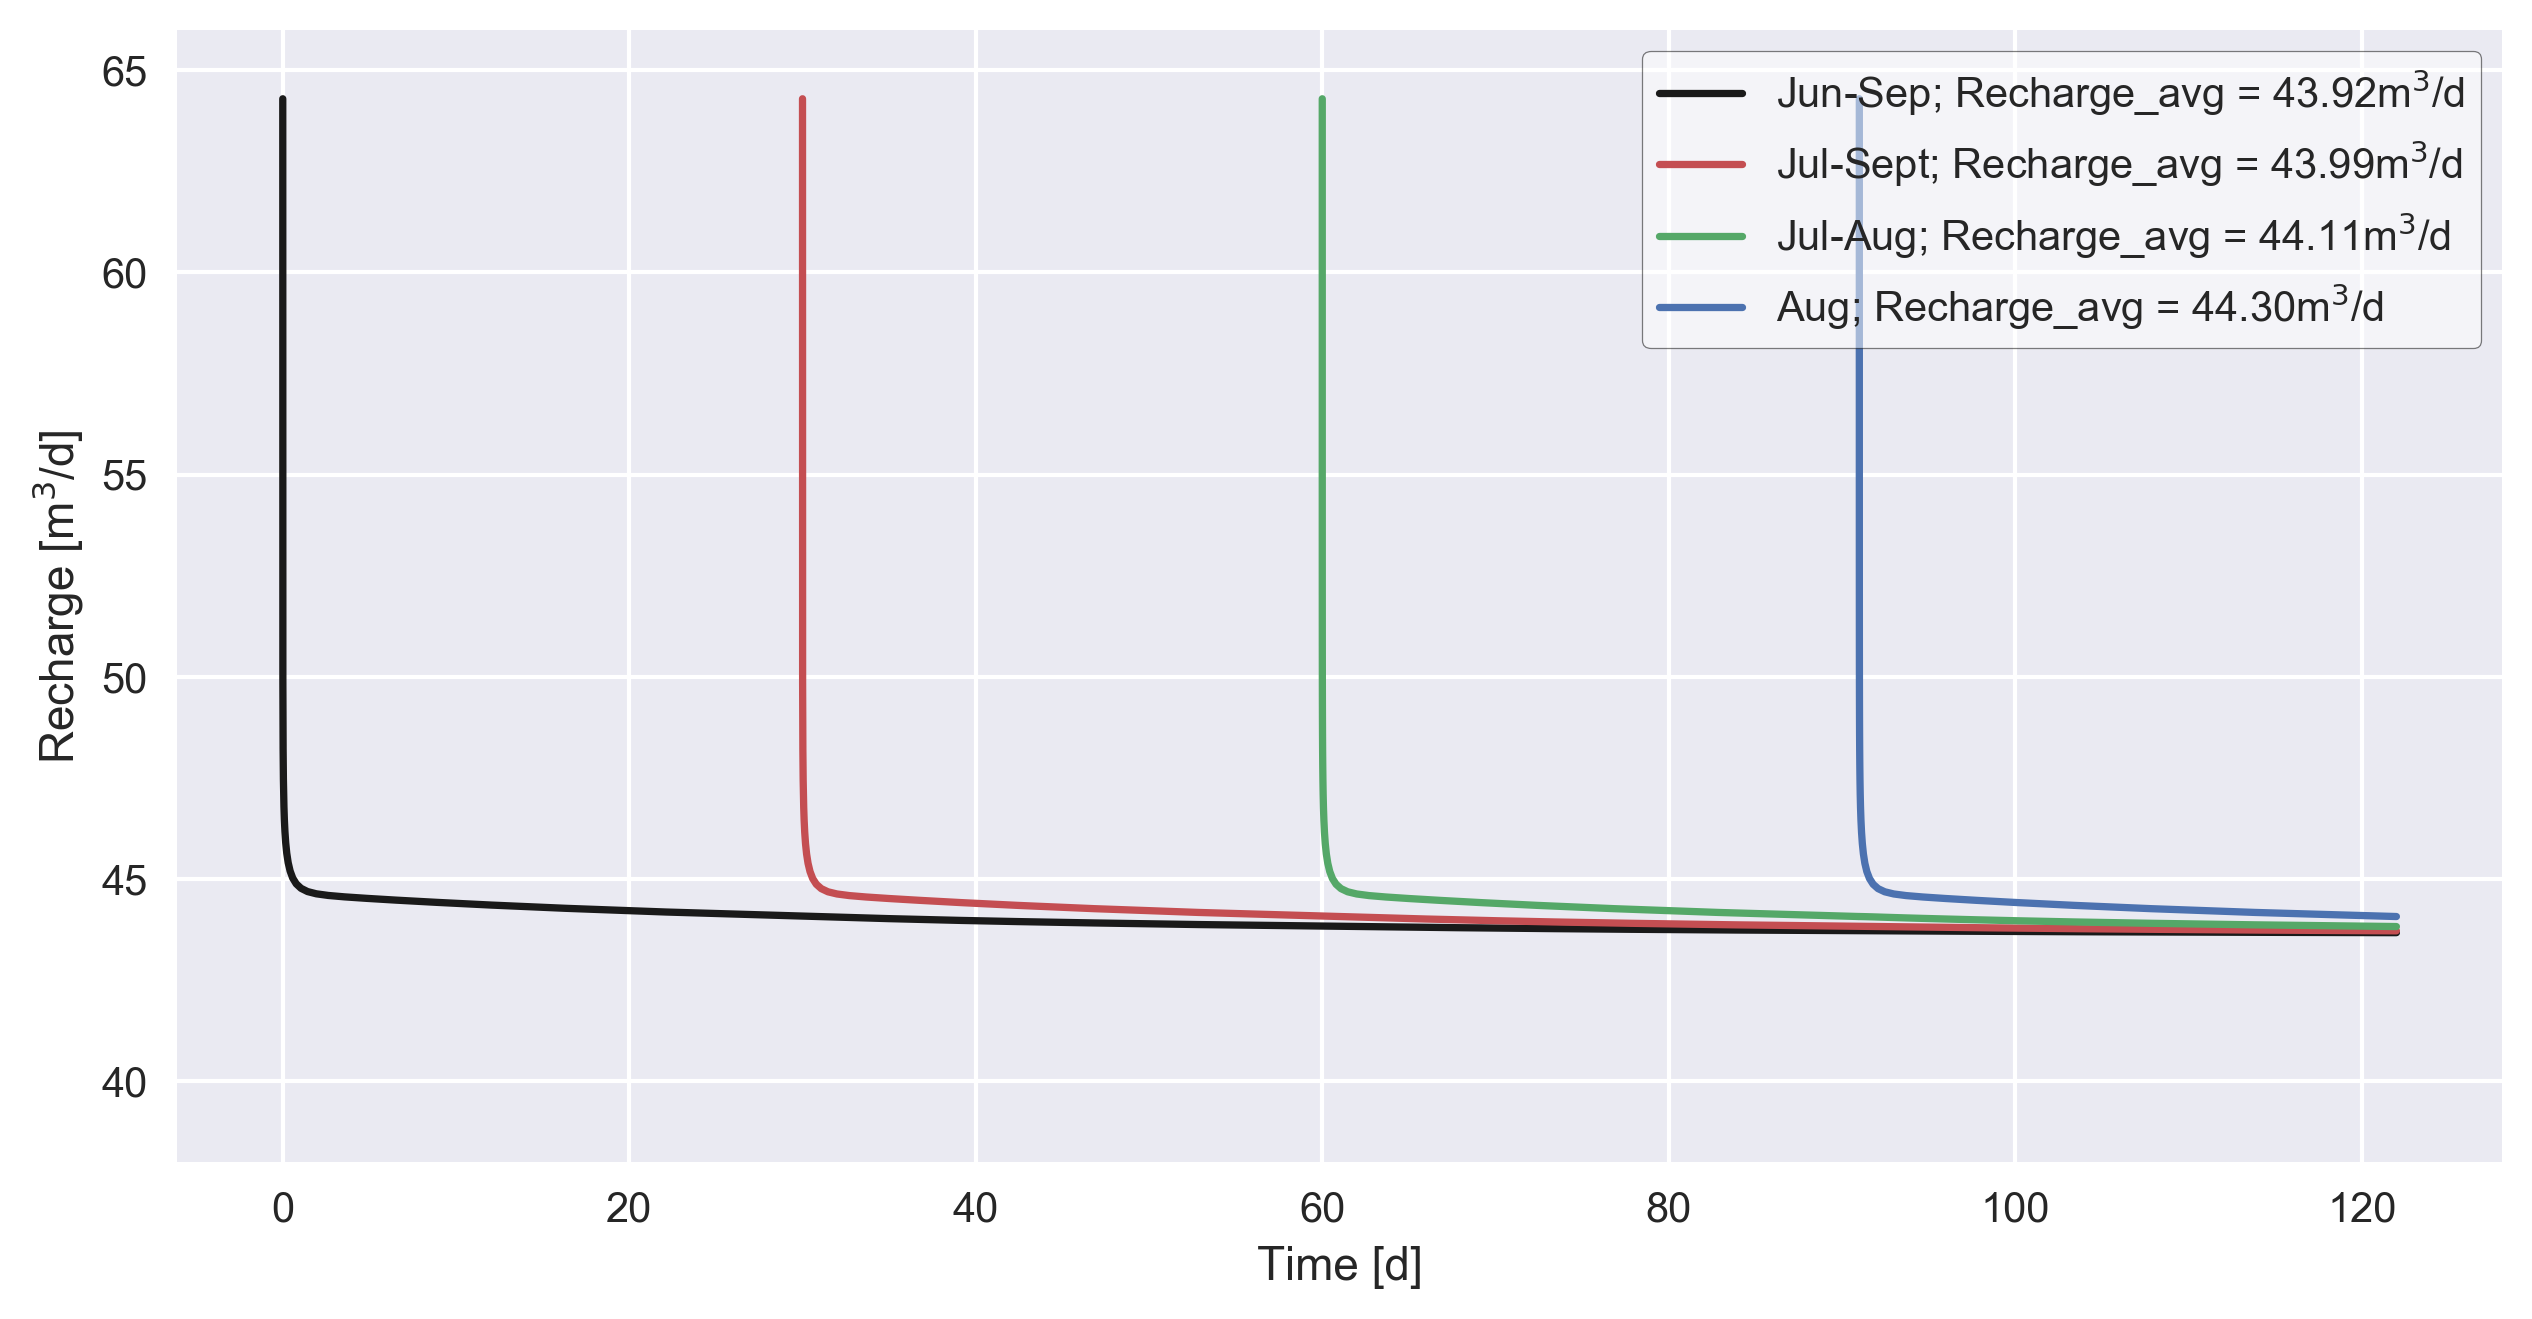
\includegraphics[width=0.7\linewidth]{Sens_delt_Sc3_recharge_time}
 \captionsetup{justification=centering} 
 \caption{Shortening wet season inundation time-span - Recharge over time - soil scenario 3}
 \label{fig:Sens_delt_Sc3_recharge_time}
\end{figure}

\begin{figure}[h!]
 \centering
 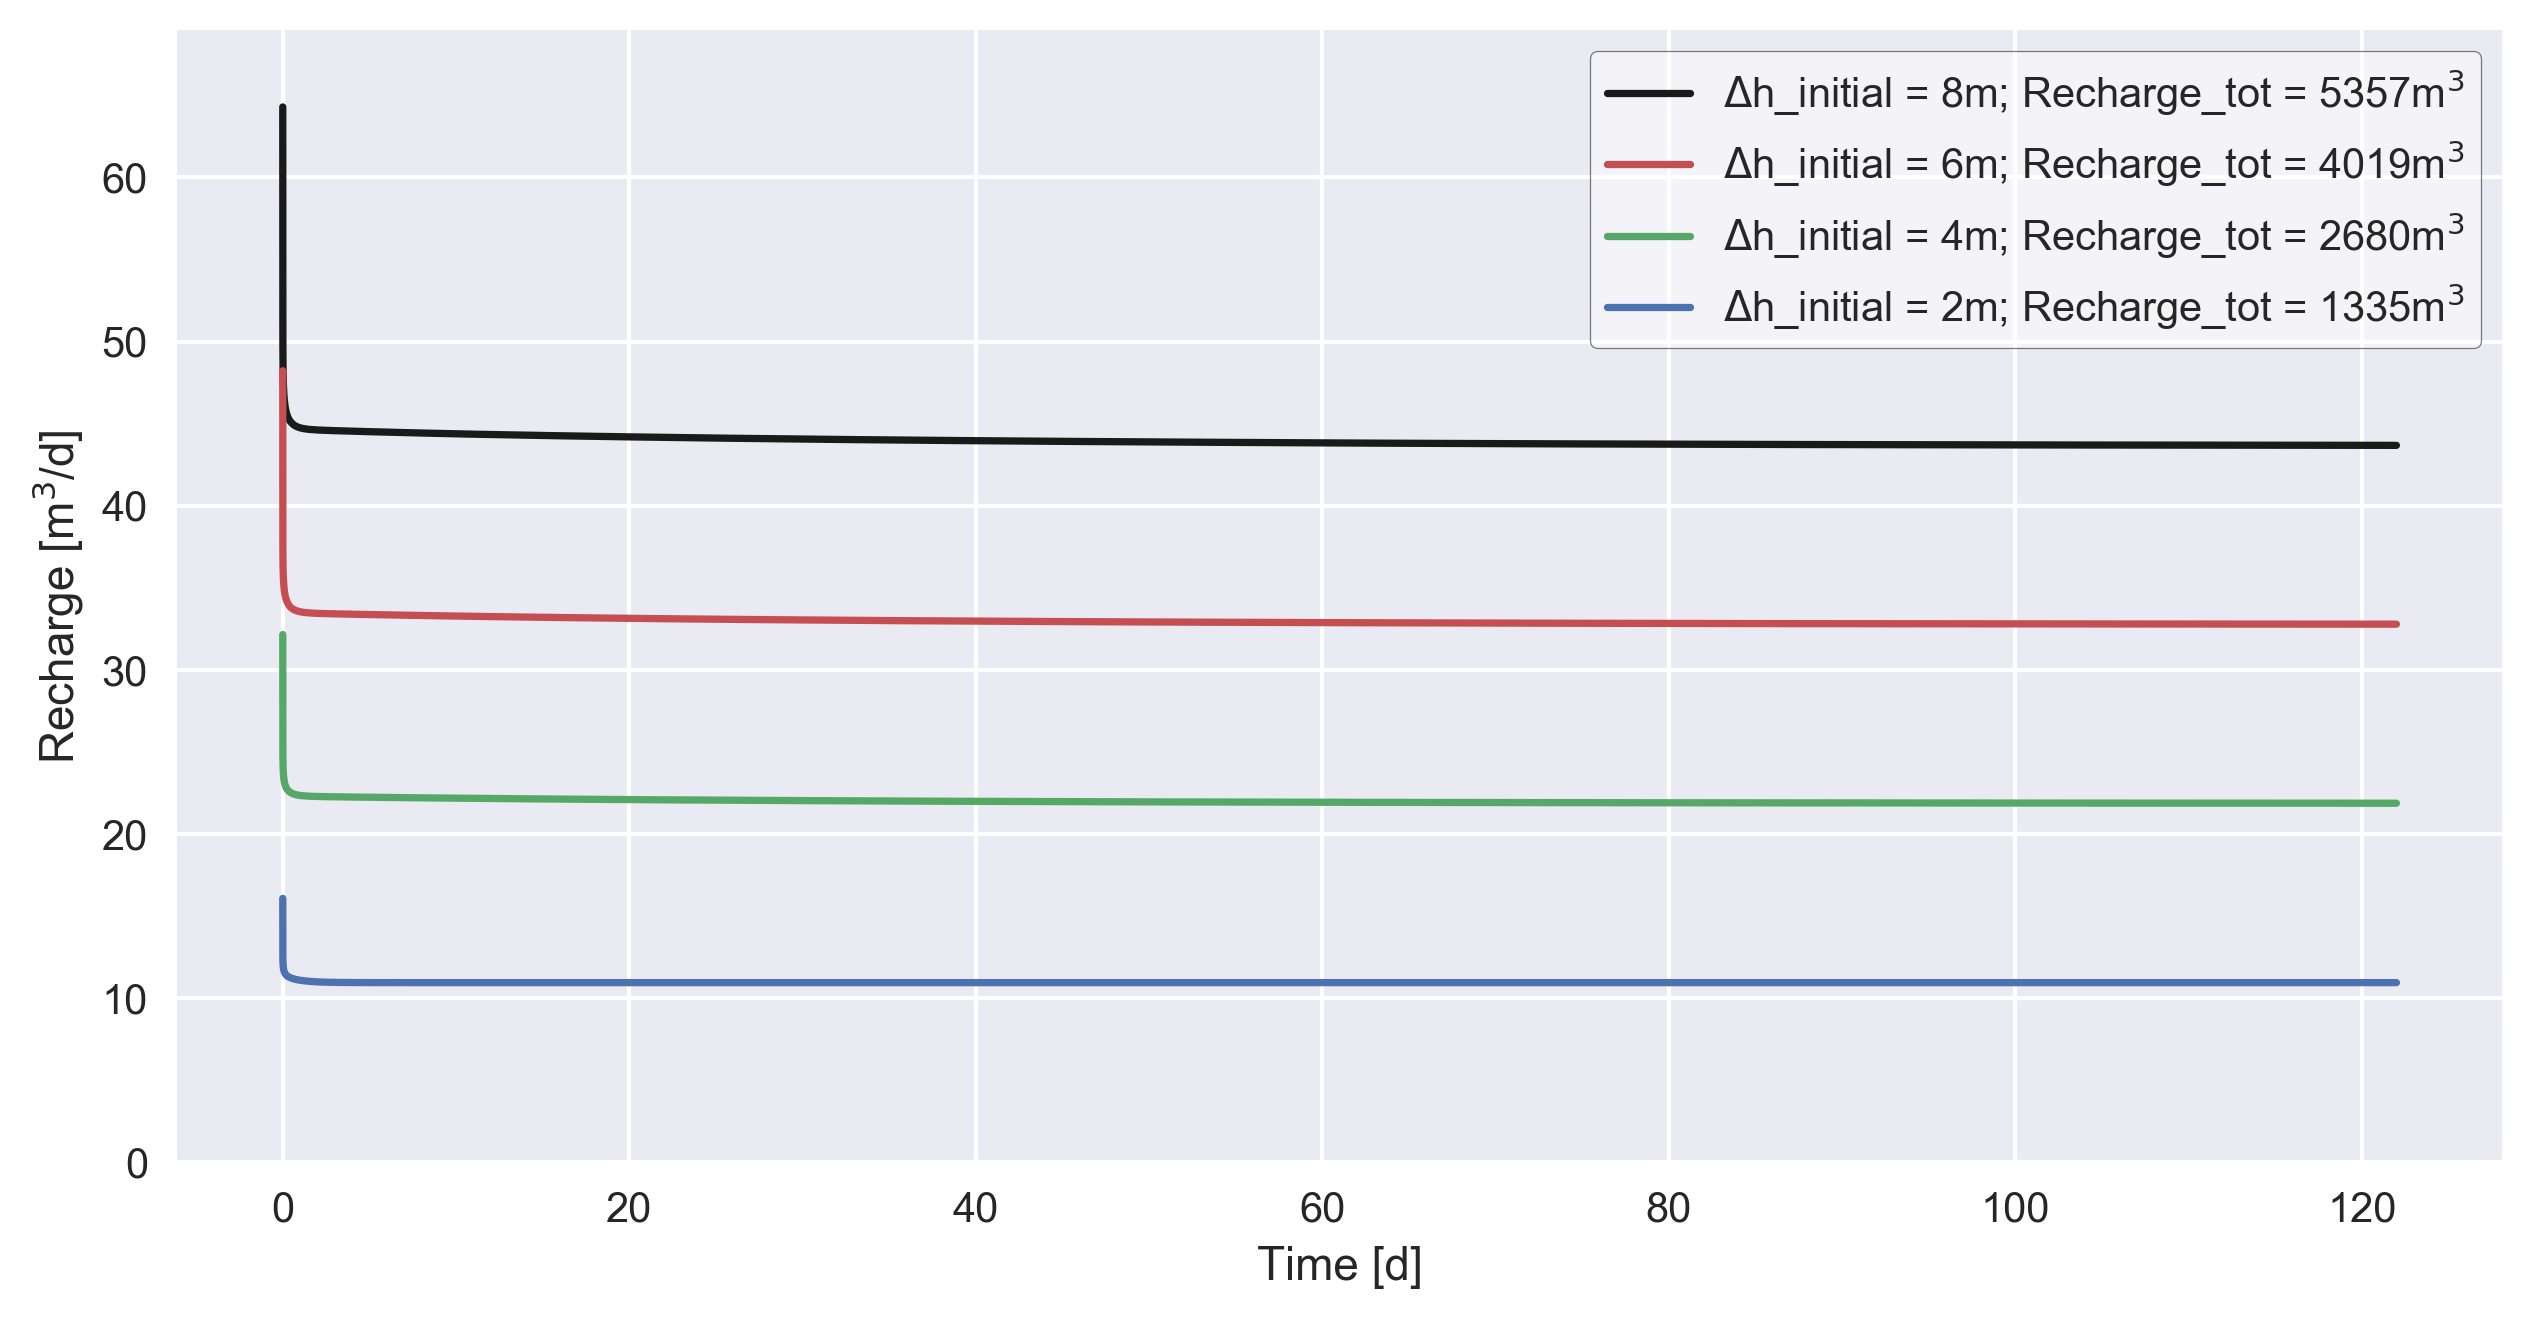
\includegraphics[width=0.7\linewidth]{Sens_delh_Sc3_recharge_time}
 \captionsetup{justification=centering} 
 \caption{Reduction wet season inundation levels - Recharge over time - soil scenario 3}
 \label{fig:Sens_delh_Sc3_recharge_time}
\end{figure}
